% Options for packages loaded elsewhere
\PassOptionsToPackage{unicode}{hyperref}
\PassOptionsToPackage{hyphens}{url}
\documentclass[
]{article}
\usepackage{xcolor}
\usepackage[margin=1in]{geometry}
\usepackage{amsmath,amssymb}
\setcounter{secnumdepth}{5}
\usepackage{iftex}
\ifPDFTeX
  \usepackage[T1]{fontenc}
  \usepackage[utf8]{inputenc}
  \usepackage{textcomp} % provide euro and other symbols
\else % if luatex or xetex
  \usepackage{unicode-math} % this also loads fontspec
  \defaultfontfeatures{Scale=MatchLowercase}
  \defaultfontfeatures[\rmfamily]{Ligatures=TeX,Scale=1}
\fi
\usepackage{lmodern}
\ifPDFTeX\else
  % xetex/luatex font selection
\fi
% Use upquote if available, for straight quotes in verbatim environments
\IfFileExists{upquote.sty}{\usepackage{upquote}}{}
\IfFileExists{microtype.sty}{% use microtype if available
  \usepackage[]{microtype}
  \UseMicrotypeSet[protrusion]{basicmath} % disable protrusion for tt fonts
}{}
\makeatletter
\@ifundefined{KOMAClassName}{% if non-KOMA class
  \IfFileExists{parskip.sty}{%
    \usepackage{parskip}
  }{% else
    \setlength{\parindent}{0pt}
    \setlength{\parskip}{6pt plus 2pt minus 1pt}}
}{% if KOMA class
  \KOMAoptions{parskip=half}}
\makeatother
\usepackage{color}
\usepackage{fancyvrb}
\newcommand{\VerbBar}{|}
\newcommand{\VERB}{\Verb[commandchars=\\\{\}]}
\DefineVerbatimEnvironment{Highlighting}{Verbatim}{commandchars=\\\{\}}
% Add ',fontsize=\small' for more characters per line
\usepackage{framed}
\definecolor{shadecolor}{RGB}{248,248,248}
\newenvironment{Shaded}{\begin{snugshade}}{\end{snugshade}}
\newcommand{\AlertTok}[1]{\textcolor[rgb]{0.94,0.16,0.16}{#1}}
\newcommand{\AnnotationTok}[1]{\textcolor[rgb]{0.56,0.35,0.01}{\textbf{\textit{#1}}}}
\newcommand{\AttributeTok}[1]{\textcolor[rgb]{0.13,0.29,0.53}{#1}}
\newcommand{\BaseNTok}[1]{\textcolor[rgb]{0.00,0.00,0.81}{#1}}
\newcommand{\BuiltInTok}[1]{#1}
\newcommand{\CharTok}[1]{\textcolor[rgb]{0.31,0.60,0.02}{#1}}
\newcommand{\CommentTok}[1]{\textcolor[rgb]{0.56,0.35,0.01}{\textit{#1}}}
\newcommand{\CommentVarTok}[1]{\textcolor[rgb]{0.56,0.35,0.01}{\textbf{\textit{#1}}}}
\newcommand{\ConstantTok}[1]{\textcolor[rgb]{0.56,0.35,0.01}{#1}}
\newcommand{\ControlFlowTok}[1]{\textcolor[rgb]{0.13,0.29,0.53}{\textbf{#1}}}
\newcommand{\DataTypeTok}[1]{\textcolor[rgb]{0.13,0.29,0.53}{#1}}
\newcommand{\DecValTok}[1]{\textcolor[rgb]{0.00,0.00,0.81}{#1}}
\newcommand{\DocumentationTok}[1]{\textcolor[rgb]{0.56,0.35,0.01}{\textbf{\textit{#1}}}}
\newcommand{\ErrorTok}[1]{\textcolor[rgb]{0.64,0.00,0.00}{\textbf{#1}}}
\newcommand{\ExtensionTok}[1]{#1}
\newcommand{\FloatTok}[1]{\textcolor[rgb]{0.00,0.00,0.81}{#1}}
\newcommand{\FunctionTok}[1]{\textcolor[rgb]{0.13,0.29,0.53}{\textbf{#1}}}
\newcommand{\ImportTok}[1]{#1}
\newcommand{\InformationTok}[1]{\textcolor[rgb]{0.56,0.35,0.01}{\textbf{\textit{#1}}}}
\newcommand{\KeywordTok}[1]{\textcolor[rgb]{0.13,0.29,0.53}{\textbf{#1}}}
\newcommand{\NormalTok}[1]{#1}
\newcommand{\OperatorTok}[1]{\textcolor[rgb]{0.81,0.36,0.00}{\textbf{#1}}}
\newcommand{\OtherTok}[1]{\textcolor[rgb]{0.56,0.35,0.01}{#1}}
\newcommand{\PreprocessorTok}[1]{\textcolor[rgb]{0.56,0.35,0.01}{\textit{#1}}}
\newcommand{\RegionMarkerTok}[1]{#1}
\newcommand{\SpecialCharTok}[1]{\textcolor[rgb]{0.81,0.36,0.00}{\textbf{#1}}}
\newcommand{\SpecialStringTok}[1]{\textcolor[rgb]{0.31,0.60,0.02}{#1}}
\newcommand{\StringTok}[1]{\textcolor[rgb]{0.31,0.60,0.02}{#1}}
\newcommand{\VariableTok}[1]{\textcolor[rgb]{0.00,0.00,0.00}{#1}}
\newcommand{\VerbatimStringTok}[1]{\textcolor[rgb]{0.31,0.60,0.02}{#1}}
\newcommand{\WarningTok}[1]{\textcolor[rgb]{0.56,0.35,0.01}{\textbf{\textit{#1}}}}
\usepackage{longtable,booktabs,array}
\usepackage{calc} % for calculating minipage widths
% Correct order of tables after \paragraph or \subparagraph
\usepackage{etoolbox}
\makeatletter
\patchcmd\longtable{\par}{\if@noskipsec\mbox{}\fi\par}{}{}
\makeatother
% Allow footnotes in longtable head/foot
\IfFileExists{footnotehyper.sty}{\usepackage{footnotehyper}}{\usepackage{footnote}}
\makesavenoteenv{longtable}
\usepackage{graphicx}
\makeatletter
\newsavebox\pandoc@box
\newcommand*\pandocbounded[1]{% scales image to fit in text height/width
  \sbox\pandoc@box{#1}%
  \Gscale@div\@tempa{\textheight}{\dimexpr\ht\pandoc@box+\dp\pandoc@box\relax}%
  \Gscale@div\@tempb{\linewidth}{\wd\pandoc@box}%
  \ifdim\@tempb\p@<\@tempa\p@\let\@tempa\@tempb\fi% select the smaller of both
  \ifdim\@tempa\p@<\p@\scalebox{\@tempa}{\usebox\pandoc@box}%
  \else\usebox{\pandoc@box}%
  \fi%
}
% Set default figure placement to htbp
\def\fps@figure{htbp}
\makeatother
\setlength{\emergencystretch}{3em} % prevent overfull lines
\providecommand{\tightlist}{%
  \setlength{\itemsep}{0pt}\setlength{\parskip}{0pt}}
\usepackage{bookmark}
\IfFileExists{xurl.sty}{\usepackage{xurl}}{} % add URL line breaks if available
\urlstyle{same}
\hypersetup{
  pdftitle={R Markdown 格式测试},
  pdfauthor={测试作者},
  hidelinks,
  pdfcreator={LaTeX via pandoc}}

\title{R Markdown 格式测试}
\author{测试作者}
\date{2025-04-11}

\begin{document}
\maketitle

{
\setcounter{tocdepth}{2}
\tableofcontents
}
\section{基本文本格式}\label{ux57faux672cux6587ux672cux683cux5f0f}

这是\textbf{粗体}文本,这是\emph{斜体}文本。

\subsection{列表示例}\label{ux5217ux8868ux793aux4f8b}

\begin{enumerate}
\def\labelenumi{\arabic{enumi}.}
\tightlist
\item
  第一项
\item
  第二项

  \begin{itemize}
  \tightlist
  \item
    子项 A
  \item
    子项 B
  \end{itemize}
\item
  第三项
\end{enumerate}

\section{数据可视化}\label{ux6570ux636eux53efux89c6ux5316}

\subsection{散点图}\label{ux6563ux70b9ux56fe}

\begin{Shaded}
\begin{Highlighting}[]
\FunctionTok{ggplot}\NormalTok{(mtcars, }\FunctionTok{aes}\NormalTok{(}\AttributeTok{x =}\NormalTok{ wt, }\AttributeTok{y =}\NormalTok{ mpg, }\AttributeTok{color =} \FunctionTok{factor}\NormalTok{(cyl))) }\SpecialCharTok{+}
  \FunctionTok{geom\_point}\NormalTok{(}\AttributeTok{size =} \DecValTok{3}\NormalTok{) }\SpecialCharTok{+}
  \FunctionTok{labs}\NormalTok{(}\AttributeTok{title =} \StringTok{"汽车重量与油耗关系"}\NormalTok{,}
       \AttributeTok{x =} \StringTok{"重量(1000磅)"}\NormalTok{,}
       \AttributeTok{y =} \StringTok{"每加仑英里数"}\NormalTok{,}
       \AttributeTok{color =} \StringTok{"气缸数"}\NormalTok{) }\SpecialCharTok{+}
  \FunctionTok{theme\_minimal}\NormalTok{()}
\end{Highlighting}
\end{Shaded}

\pandocbounded{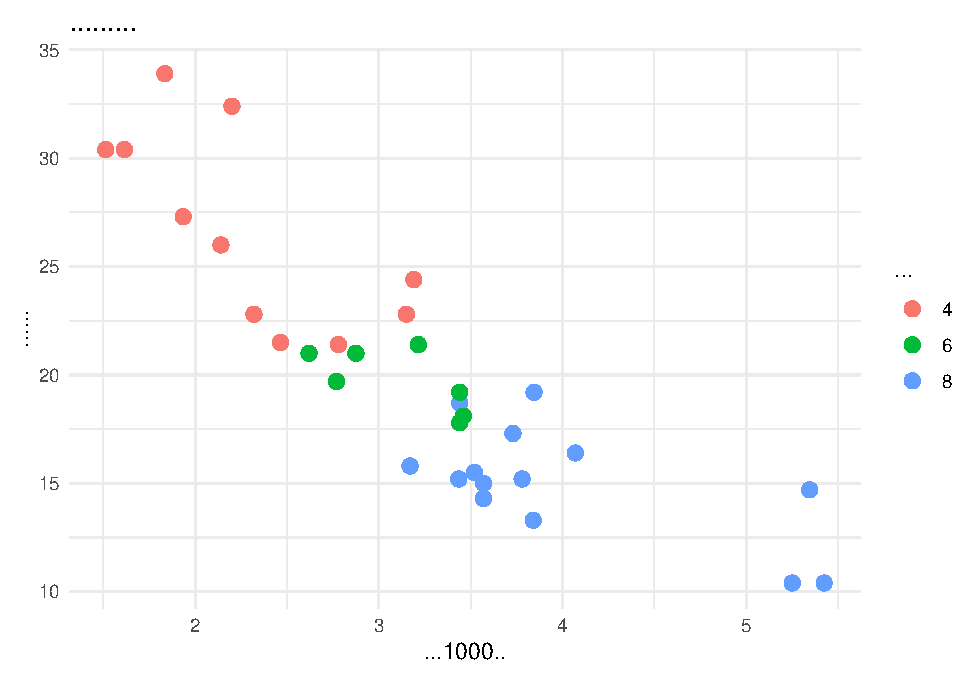
\includegraphics[keepaspectratio]{/github/workspace/_output/test_formats_files/figure-latex/scatter-1.pdf}}

\subsection{箱线图}\label{ux7bb1ux7ebfux56fe}

\begin{Shaded}
\begin{Highlighting}[]
\FunctionTok{ggplot}\NormalTok{(mtcars, }\FunctionTok{aes}\NormalTok{(}\AttributeTok{x =} \FunctionTok{factor}\NormalTok{(cyl), }\AttributeTok{y =}\NormalTok{ mpg, }\AttributeTok{fill =} \FunctionTok{factor}\NormalTok{(cyl))) }\SpecialCharTok{+}
  \FunctionTok{geom\_boxplot}\NormalTok{() }\SpecialCharTok{+}
  \FunctionTok{labs}\NormalTok{(}\AttributeTok{title =} \StringTok{"不同气缸数的油耗分布"}\NormalTok{,}
       \AttributeTok{x =} \StringTok{"气缸数"}\NormalTok{,}
       \AttributeTok{y =} \StringTok{"每加仑英里数"}\NormalTok{,}
       \AttributeTok{fill =} \StringTok{"气缸数"}\NormalTok{) }\SpecialCharTok{+}
  \FunctionTok{theme\_minimal}\NormalTok{()}
\end{Highlighting}
\end{Shaded}

\pandocbounded{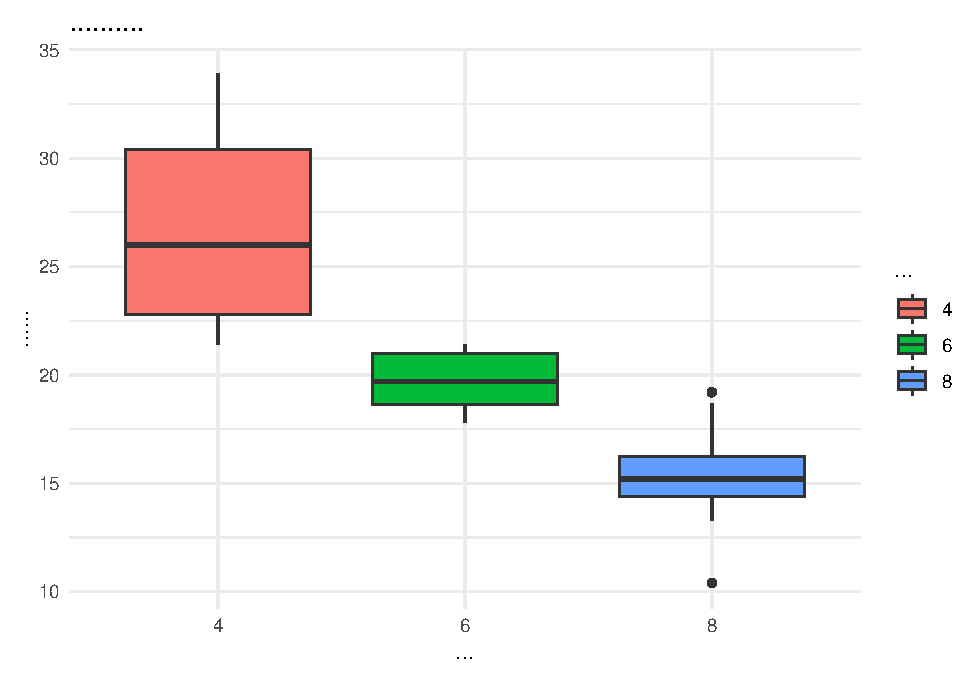
\includegraphics[keepaspectratio]{/github/workspace/_output/test_formats_files/figure-latex/boxplot-1.pdf}}

\section{表格}\label{ux8868ux683c}

\subsection{基本表格}\label{ux57faux672cux8868ux683c}

\begin{Shaded}
\begin{Highlighting}[]
\NormalTok{knitr}\SpecialCharTok{::}\FunctionTok{kable}\NormalTok{(}\FunctionTok{head}\NormalTok{(mtcars[, }\DecValTok{1}\SpecialCharTok{:}\DecValTok{5}\NormalTok{]), }
             \AttributeTok{caption =} \StringTok{"mtcars 数据集前6行"}\NormalTok{,}
             \AttributeTok{booktabs =} \ConstantTok{TRUE}\NormalTok{)}
\end{Highlighting}
\end{Shaded}

\begin{longtable}[]{@{}lrrrrr@{}}
\caption{mtcars 数据集前6行}\tabularnewline
\toprule\noalign{}
& mpg & cyl & disp & hp & drat \\
\midrule\noalign{}
\endfirsthead
\toprule\noalign{}
& mpg & cyl & disp & hp & drat \\
\midrule\noalign{}
\endhead
\bottomrule\noalign{}
\endlastfoot
Mazda RX4 & 21.0 & 6 & 160 & 110 & 3.90 \\
Mazda RX4 Wag & 21.0 & 6 & 160 & 110 & 3.90 \\
Datsun 710 & 22.8 & 4 & 108 & 93 & 3.85 \\
Hornet 4 Drive & 21.4 & 6 & 258 & 110 & 3.08 \\
Hornet Sportabout & 18.7 & 8 & 360 & 175 & 3.15 \\
Valiant & 18.1 & 6 & 225 & 105 & 2.76 \\
\end{longtable}

\subsection{统计摘要}\label{ux7edfux8ba1ux6458ux8981}

\begin{Shaded}
\begin{Highlighting}[]
\NormalTok{summary\_stats }\OtherTok{\textless{}{-}} \FunctionTok{aggregate}\NormalTok{(mpg }\SpecialCharTok{\textasciitilde{}}\NormalTok{ cyl, }\AttributeTok{data =}\NormalTok{ mtcars, }
                         \AttributeTok{FUN =} \ControlFlowTok{function}\NormalTok{(x) }\FunctionTok{c}\NormalTok{(}\AttributeTok{mean =} \FunctionTok{mean}\NormalTok{(x), }
                                           \AttributeTok{sd =} \FunctionTok{sd}\NormalTok{(x)))}
\NormalTok{knitr}\SpecialCharTok{::}\FunctionTok{kable}\NormalTok{(summary\_stats,}
             \AttributeTok{caption =} \StringTok{"不同气缸数的油耗统计"}\NormalTok{,}
             \AttributeTok{booktabs =} \ConstantTok{TRUE}\NormalTok{)}
\end{Highlighting}
\end{Shaded}

\begin{verbatim}
## Warning in `[<-.data.frame`(`*tmp*`, , isn, value = structure(list(cyl =
## structure(c("4", : provided 3 variables to replace 2 variables
\end{verbatim}

\begin{longtable}[]{@{}rr@{}}
\caption{不同气缸数的油耗统计}\tabularnewline
\toprule\noalign{}
cyl & mpg \\
\midrule\noalign{}
\endfirsthead
\toprule\noalign{}
cyl & mpg \\
\midrule\noalign{}
\endhead
\bottomrule\noalign{}
\endlastfoot
4 & 26.663636 \\
6 & 19.742857 \\
8 & 15.100000 \\
\end{longtable}

\section{数学公式}\label{ux6570ux5b66ux516cux5f0f}

行内公式:当 \(x \to \infty\) 时,\(e^{-x} \to 0\)

显示公式:

\[
f(x) = \frac{1}{\sigma\sqrt{2\pi}} e^{-\frac{(x-\mu)^2}{2\sigma^2}}
\]

\section{代码示例}\label{ux4ee3ux7801ux793aux4f8b}

\begin{Shaded}
\begin{Highlighting}[]
\NormalTok{fibonacci }\OtherTok{\textless{}{-}} \ControlFlowTok{function}\NormalTok{(n) \{}
  \ControlFlowTok{if}\NormalTok{ (n }\SpecialCharTok{\textless{}=} \DecValTok{1}\NormalTok{) }\FunctionTok{return}\NormalTok{(n)}
\NormalTok{  fib }\OtherTok{\textless{}{-}} \FunctionTok{numeric}\NormalTok{(n}\SpecialCharTok{+}\DecValTok{1}\NormalTok{)}
\NormalTok{  fib[}\DecValTok{1}\NormalTok{] }\OtherTok{\textless{}{-}} \DecValTok{0}
\NormalTok{  fib[}\DecValTok{2}\NormalTok{] }\OtherTok{\textless{}{-}} \DecValTok{1}
  \ControlFlowTok{for}\NormalTok{ (i }\ControlFlowTok{in} \DecValTok{3}\SpecialCharTok{:}\NormalTok{(n}\SpecialCharTok{+}\DecValTok{1}\NormalTok{)) \{}
\NormalTok{    fib[i] }\OtherTok{\textless{}{-}}\NormalTok{ fib[i}\DecValTok{{-}1}\NormalTok{] }\SpecialCharTok{+}\NormalTok{ fib[i}\DecValTok{{-}2}\NormalTok{]}
\NormalTok{  \}}
  \FunctionTok{return}\NormalTok{(fib[n}\SpecialCharTok{+}\DecValTok{1}\NormalTok{])}
\NormalTok{\}}

\CommentTok{\# 测试函数}
\FunctionTok{sapply}\NormalTok{(}\DecValTok{0}\SpecialCharTok{:}\DecValTok{5}\NormalTok{, fibonacci)}
\end{Highlighting}
\end{Shaded}

\begin{verbatim}
## [1] 0 1 1 2 3 5
\end{verbatim}

\end{document}
